% Created by tikzDevice version 0.7.0 on 2015-09-21 12:44:19
% !TEX encoding = UTF-8 Unicode
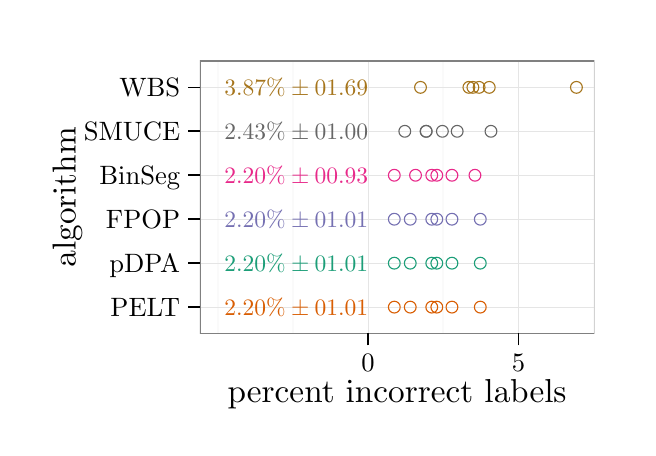
\begin{tikzpicture}[x=1pt,y=1pt]
\definecolor[named]{fillColor}{rgb}{1.00,1.00,1.00}
\path[use as bounding box,fill=fillColor,fill opacity=0.00] (0,0) rectangle (216.81,144.54);
\begin{scope}
\path[clip] (  0.00,  0.00) rectangle (216.81,144.54);
\definecolor[named]{drawColor}{rgb}{1.00,1.00,1.00}
\definecolor[named]{fillColor}{rgb}{1.00,1.00,1.00}

\path[draw=drawColor,line width= 0.6pt,line join=round,line cap=round,fill=fillColor] ( -0.00,  0.00) rectangle (216.81,144.54);
\end{scope}
\begin{scope}
\path[clip] ( 62.21, 34.03) rectangle (204.76,132.50);
\definecolor[named]{fillColor}{rgb}{1.00,1.00,1.00}

\path[fill=fillColor] ( 62.21, 34.03) rectangle (204.76,132.50);
\definecolor[named]{drawColor}{rgb}{0.98,0.98,0.98}

\path[draw=drawColor,line width= 0.6pt,line join=round] ( 68.69, 34.03) --
	( 68.69,132.50);

\path[draw=drawColor,line width= 0.6pt,line join=round] ( 95.86, 34.03) --
	( 95.86,132.50);

\path[draw=drawColor,line width= 0.6pt,line join=round] (150.18, 34.03) --
	(150.18,132.50);

\path[draw=drawColor,line width= 0.6pt,line join=round] (204.51, 34.03) --
	(204.51,132.50);
\definecolor[named]{drawColor}{rgb}{0.90,0.90,0.90}

\path[draw=drawColor,line width= 0.2pt,line join=round] ( 62.21, 43.56) --
	(204.76, 43.56);

\path[draw=drawColor,line width= 0.2pt,line join=round] ( 62.21, 59.44) --
	(204.76, 59.44);

\path[draw=drawColor,line width= 0.2pt,line join=round] ( 62.21, 75.32) --
	(204.76, 75.32);

\path[draw=drawColor,line width= 0.2pt,line join=round] ( 62.21, 91.21) --
	(204.76, 91.21);

\path[draw=drawColor,line width= 0.2pt,line join=round] ( 62.21,107.09) --
	(204.76,107.09);

\path[draw=drawColor,line width= 0.2pt,line join=round] ( 62.21,122.97) --
	(204.76,122.97);

\path[draw=drawColor,line width= 0.2pt,line join=round] (123.02, 34.03) --
	(123.02,132.50);

\path[draw=drawColor,line width= 0.2pt,line join=round] (177.35, 34.03) --
	(177.35,132.50);
\definecolor[named]{drawColor}{rgb}{0.85,0.37,0.01}

\node[text=drawColor,anchor=base east,inner sep=0pt, outer sep=0pt, scale=  0.85] at (123.02, 40.63) {$2.20\% \pm 01.01$};
\definecolor[named]{drawColor}{rgb}{0.11,0.62,0.47}

\node[text=drawColor,anchor=base east,inner sep=0pt, outer sep=0pt, scale=  0.85] at (123.02, 56.52) {$2.20\% \pm 01.01$};
\definecolor[named]{drawColor}{rgb}{0.46,0.44,0.70}

\node[text=drawColor,anchor=base east,inner sep=0pt, outer sep=0pt, scale=  0.85] at (123.02, 72.40) {$2.20\% \pm 01.01$};
\definecolor[named]{drawColor}{rgb}{0.91,0.16,0.54}

\node[text=drawColor,anchor=base east,inner sep=0pt, outer sep=0pt, scale=  0.85] at (123.02, 88.28) {$2.20\% \pm 00.93$};
\definecolor[named]{drawColor}{rgb}{0.40,0.40,0.40}

\node[text=drawColor,anchor=base east,inner sep=0pt, outer sep=0pt, scale=  0.85] at (123.02,104.16) {$2.43\% \pm 01.00$};
\definecolor[named]{drawColor}{rgb}{0.65,0.46,0.11}

\node[text=drawColor,anchor=base east,inner sep=0pt, outer sep=0pt, scale=  0.85] at (123.02,120.04) {$3.87\% \pm 01.69$};
\definecolor[named]{drawColor}{rgb}{0.85,0.37,0.01}

\path[draw=drawColor,line width= 0.4pt,line join=round,line cap=round] (146.02, 43.56) circle (  2.13);

\path[draw=drawColor,line width= 0.4pt,line join=round,line cap=round] (153.31, 43.56) circle (  2.13);

\path[draw=drawColor,line width= 0.4pt,line join=round,line cap=round] (132.48, 43.56) circle (  2.13);

\path[draw=drawColor,line width= 0.4pt,line join=round,line cap=round] (147.84, 43.56) circle (  2.13);

\path[draw=drawColor,line width= 0.4pt,line join=round,line cap=round] (138.24, 43.56) circle (  2.13);

\path[draw=drawColor,line width= 0.4pt,line join=round,line cap=round] (163.55, 43.56) circle (  2.13);
\definecolor[named]{drawColor}{rgb}{0.11,0.62,0.47}

\path[draw=drawColor,line width= 0.4pt,line join=round,line cap=round] (146.02, 59.44) circle (  2.13);

\path[draw=drawColor,line width= 0.4pt,line join=round,line cap=round] (153.31, 59.44) circle (  2.13);

\path[draw=drawColor,line width= 0.4pt,line join=round,line cap=round] (132.48, 59.44) circle (  2.13);

\path[draw=drawColor,line width= 0.4pt,line join=round,line cap=round] (147.84, 59.44) circle (  2.13);

\path[draw=drawColor,line width= 0.4pt,line join=round,line cap=round] (138.24, 59.44) circle (  2.13);

\path[draw=drawColor,line width= 0.4pt,line join=round,line cap=round] (163.55, 59.44) circle (  2.13);
\definecolor[named]{drawColor}{rgb}{0.46,0.44,0.70}

\path[draw=drawColor,line width= 0.4pt,line join=round,line cap=round] (146.02, 75.32) circle (  2.13);

\path[draw=drawColor,line width= 0.4pt,line join=round,line cap=round] (153.31, 75.32) circle (  2.13);

\path[draw=drawColor,line width= 0.4pt,line join=round,line cap=round] (132.48, 75.32) circle (  2.13);

\path[draw=drawColor,line width= 0.4pt,line join=round,line cap=round] (147.84, 75.32) circle (  2.13);

\path[draw=drawColor,line width= 0.4pt,line join=round,line cap=round] (138.24, 75.32) circle (  2.13);

\path[draw=drawColor,line width= 0.4pt,line join=round,line cap=round] (163.55, 75.32) circle (  2.13);
\definecolor[named]{drawColor}{rgb}{0.91,0.16,0.54}

\path[draw=drawColor,line width= 0.4pt,line join=round,line cap=round] (146.02, 91.21) circle (  2.13);

\path[draw=drawColor,line width= 0.4pt,line join=round,line cap=round] (153.31, 91.21) circle (  2.13);

\path[draw=drawColor,line width= 0.4pt,line join=round,line cap=round] (132.48, 91.21) circle (  2.13);

\path[draw=drawColor,line width= 0.4pt,line join=round,line cap=round] (147.84, 91.21) circle (  2.13);

\path[draw=drawColor,line width= 0.4pt,line join=round,line cap=round] (140.15, 91.21) circle (  2.13);

\path[draw=drawColor,line width= 0.4pt,line join=round,line cap=round] (161.62, 91.21) circle (  2.13);
\definecolor[named]{drawColor}{rgb}{0.40,0.40,0.40}

\path[draw=drawColor,line width= 0.4pt,line join=round,line cap=round] (149.85,107.09) circle (  2.13);

\path[draw=drawColor,line width= 0.4pt,line join=round,line cap=round] (155.20,107.09) circle (  2.13);

\path[draw=drawColor,line width= 0.4pt,line join=round,line cap=round] (136.27,107.09) circle (  2.13);

\path[draw=drawColor,line width= 0.4pt,line join=round,line cap=round] (144.02,107.09) circle (  2.13);

\path[draw=drawColor,line width= 0.4pt,line join=round,line cap=round] (143.95,107.09) circle (  2.13);

\path[draw=drawColor,line width= 0.4pt,line join=round,line cap=round] (167.41,107.09) circle (  2.13);
\definecolor[named]{drawColor}{rgb}{0.65,0.46,0.11}

\path[draw=drawColor,line width= 0.4pt,line join=round,line cap=round] (159.43,122.97) circle (  2.13);

\path[draw=drawColor,line width= 0.4pt,line join=round,line cap=round] (160.88,122.97) circle (  2.13);

\path[draw=drawColor,line width= 0.4pt,line join=round,line cap=round] (141.95,122.97) circle (  2.13);

\path[draw=drawColor,line width= 0.4pt,line join=round,line cap=round] (163.12,122.97) circle (  2.13);

\path[draw=drawColor,line width= 0.4pt,line join=round,line cap=round] (166.79,122.97) circle (  2.13);

\path[draw=drawColor,line width= 0.4pt,line join=round,line cap=round] (198.29,122.97) circle (  2.13);
\definecolor[named]{drawColor}{rgb}{0.50,0.50,0.50}

\path[draw=drawColor,line width= 0.6pt,line join=round,line cap=round] ( 62.21, 34.03) rectangle (204.76,132.50);
\end{scope}
\begin{scope}
\path[clip] (  0.00,  0.00) rectangle (216.81,144.54);
\definecolor[named]{drawColor}{rgb}{0.00,0.00,0.00}

\node[text=drawColor,anchor=base east,inner sep=0pt, outer sep=0pt, scale=  0.96] at ( 55.10, 40.26) {PELT};

\node[text=drawColor,anchor=base east,inner sep=0pt, outer sep=0pt, scale=  0.96] at ( 55.10, 56.14) {pDPA};

\node[text=drawColor,anchor=base east,inner sep=0pt, outer sep=0pt, scale=  0.96] at ( 55.10, 72.02) {FPOP};

\node[text=drawColor,anchor=base east,inner sep=0pt, outer sep=0pt, scale=  0.96] at ( 55.10, 87.90) {BinSeg};

\node[text=drawColor,anchor=base east,inner sep=0pt, outer sep=0pt, scale=  0.96] at ( 55.10,103.78) {SMUCE};

\node[text=drawColor,anchor=base east,inner sep=0pt, outer sep=0pt, scale=  0.96] at ( 55.10,119.66) {WBS};
\end{scope}
\begin{scope}
\path[clip] (  0.00,  0.00) rectangle (216.81,144.54);
\definecolor[named]{drawColor}{rgb}{0.00,0.00,0.00}

\path[draw=drawColor,line width= 0.6pt,line join=round] ( 57.95, 43.56) --
	( 62.21, 43.56);

\path[draw=drawColor,line width= 0.6pt,line join=round] ( 57.95, 59.44) --
	( 62.21, 59.44);

\path[draw=drawColor,line width= 0.6pt,line join=round] ( 57.95, 75.32) --
	( 62.21, 75.32);

\path[draw=drawColor,line width= 0.6pt,line join=round] ( 57.95, 91.21) --
	( 62.21, 91.21);

\path[draw=drawColor,line width= 0.6pt,line join=round] ( 57.95,107.09) --
	( 62.21,107.09);

\path[draw=drawColor,line width= 0.6pt,line join=round] ( 57.95,122.97) --
	( 62.21,122.97);
\end{scope}
\begin{scope}
\path[clip] (  0.00,  0.00) rectangle (216.81,144.54);
\definecolor[named]{drawColor}{rgb}{0.00,0.00,0.00}

\path[draw=drawColor,line width= 0.6pt,line join=round] (123.02, 29.77) --
	(123.02, 34.03);

\path[draw=drawColor,line width= 0.6pt,line join=round] (177.35, 29.77) --
	(177.35, 34.03);
\end{scope}
\begin{scope}
\path[clip] (  0.00,  0.00) rectangle (216.81,144.54);
\definecolor[named]{drawColor}{rgb}{0.00,0.00,0.00}

\node[text=drawColor,anchor=base,inner sep=0pt, outer sep=0pt, scale=  0.96] at (123.02, 20.31) {0};

\node[text=drawColor,anchor=base,inner sep=0pt, outer sep=0pt, scale=  0.96] at (177.35, 20.31) {5};
\end{scope}
\begin{scope}
\path[clip] (  0.00,  0.00) rectangle (216.81,144.54);
\definecolor[named]{drawColor}{rgb}{0.00,0.00,0.00}

\node[text=drawColor,anchor=base,inner sep=0pt, outer sep=0pt, scale=  1.20] at (133.49,  9.03) {percent incorrect labels};
\end{scope}
\begin{scope}
\path[clip] (  0.00,  0.00) rectangle (216.81,144.54);
\definecolor[named]{drawColor}{rgb}{0.00,0.00,0.00}

\node[text=drawColor,rotate= 90.00,anchor=base,inner sep=0pt, outer sep=0pt, scale=  1.20] at ( 17.30, 83.26) {algorithm};
\end{scope}
\end{tikzpicture}
